\section{Ejercicio 1: Conexión a datos de Power BI - Tarea 2: Conectarse a Datos Existentes en Azure} 

1. Open SQL Server Management Studio from the taskbar, and then connect to the MIA-SQL database engine instance by using Windows authentication.\\
2. On the File menu, point to Open, click Project/Solution, browse to the D:/Labfiles/Lab06/Starter/Project folder, and then double-click Project.ssmssln.

	\begin{center}
	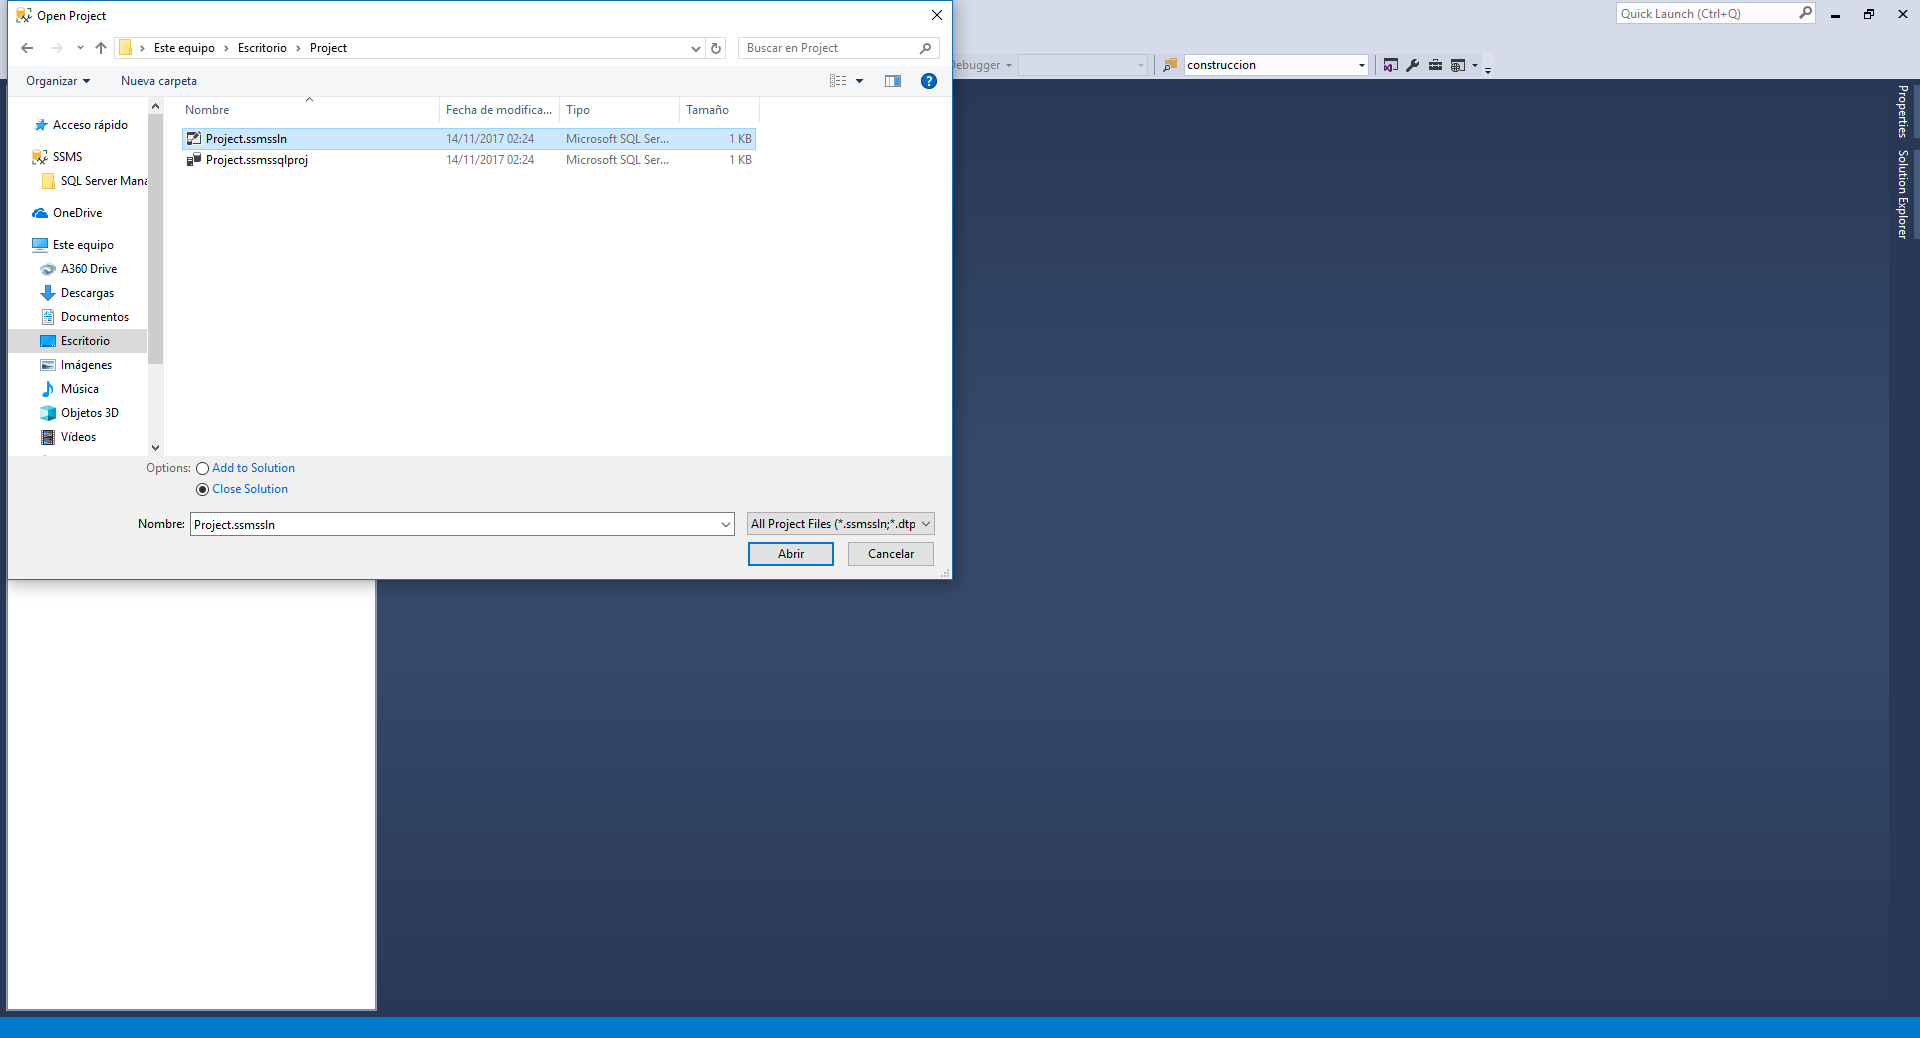
\includegraphics[width=17cm]{./Imagenes/Ejercicio1/Tarea2/1}
	\end{center}	

3. In Solution Explorer, expand Queries, and then double-click Lab Exercise 1.sql.\\

	\begin{center}
	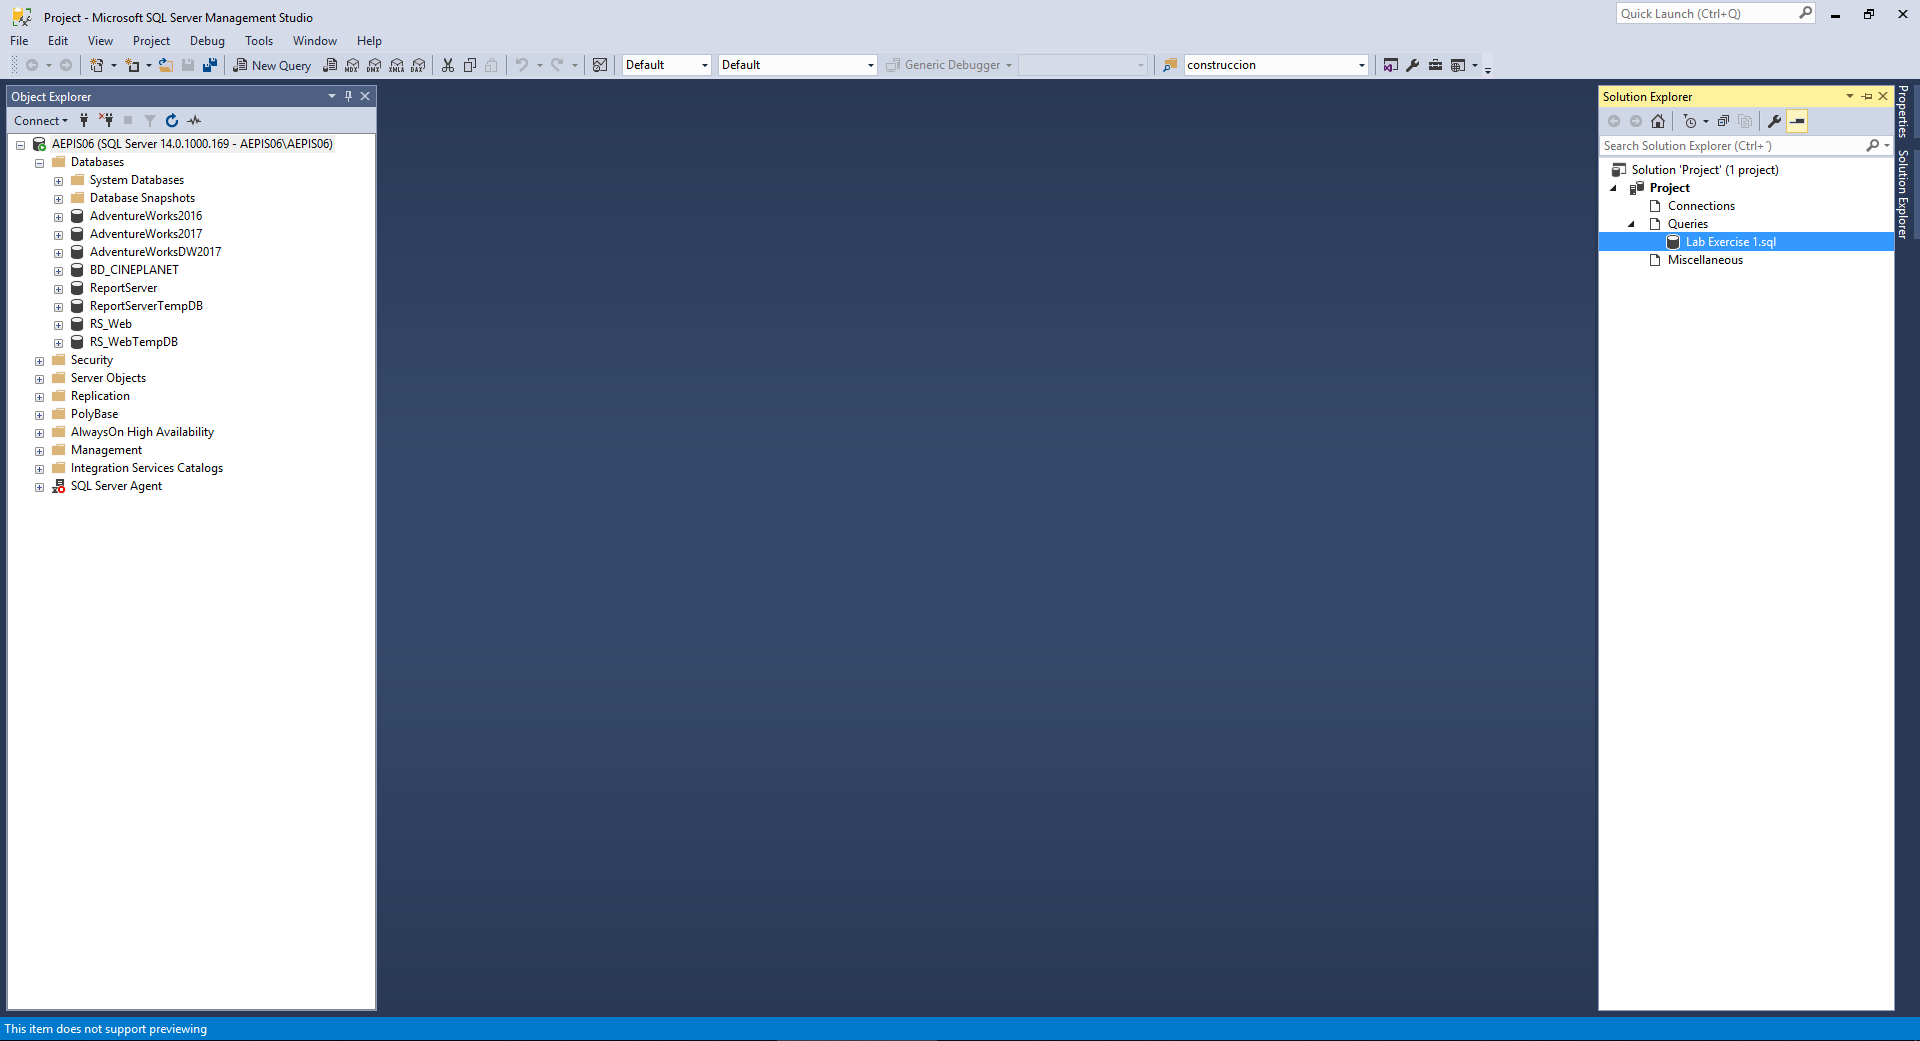
\includegraphics[width=17cm]{./Imagenes/Ejercicio1/Tarea2/2}
	\end{center}	

4. On the Desktop, double-click Power BI Desktop.\\
5. In the Power BI Desktop window, click Get Data.\\

	\begin{center}
	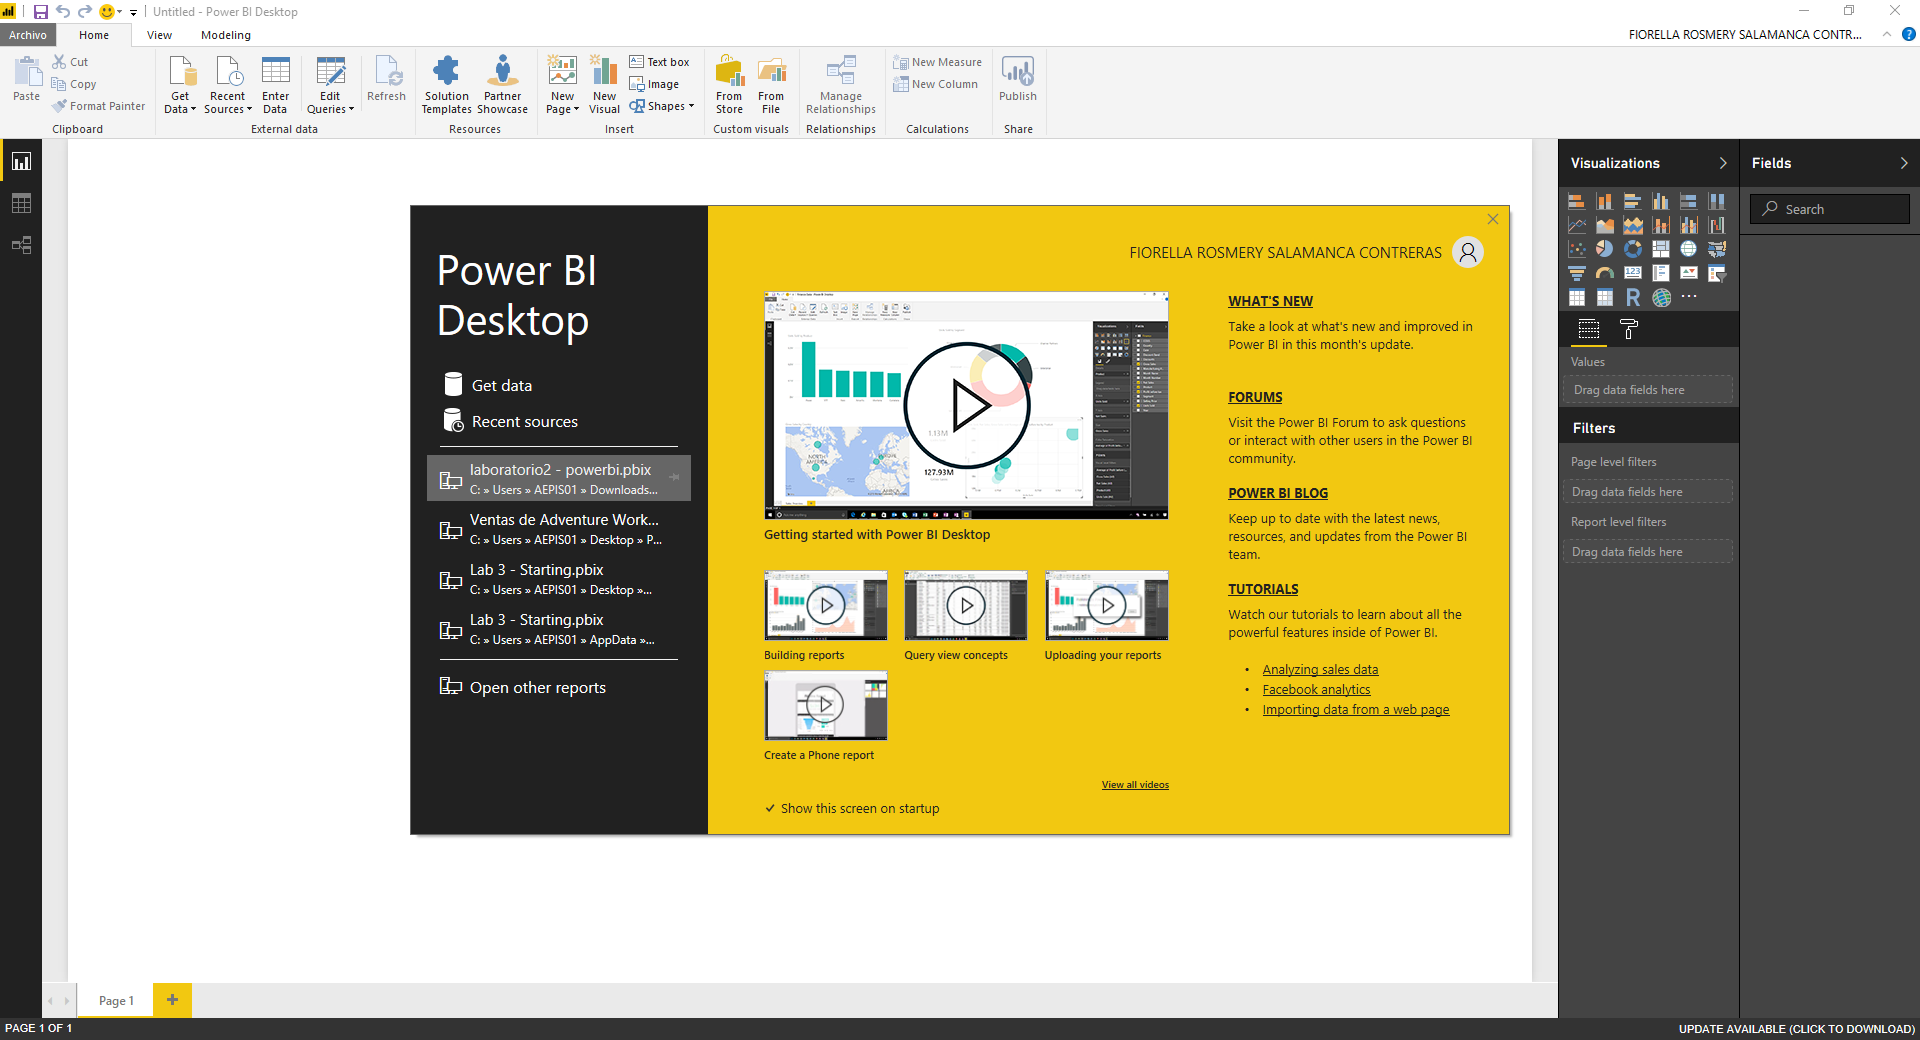
\includegraphics[width=17cm]{./Imagenes/Ejercicio1/Tarea2/3}
	\end{center}	

6. In the Get Data dialog box, click Microsoft Azure SQL database, and then click Connect\\

	\begin{center}
	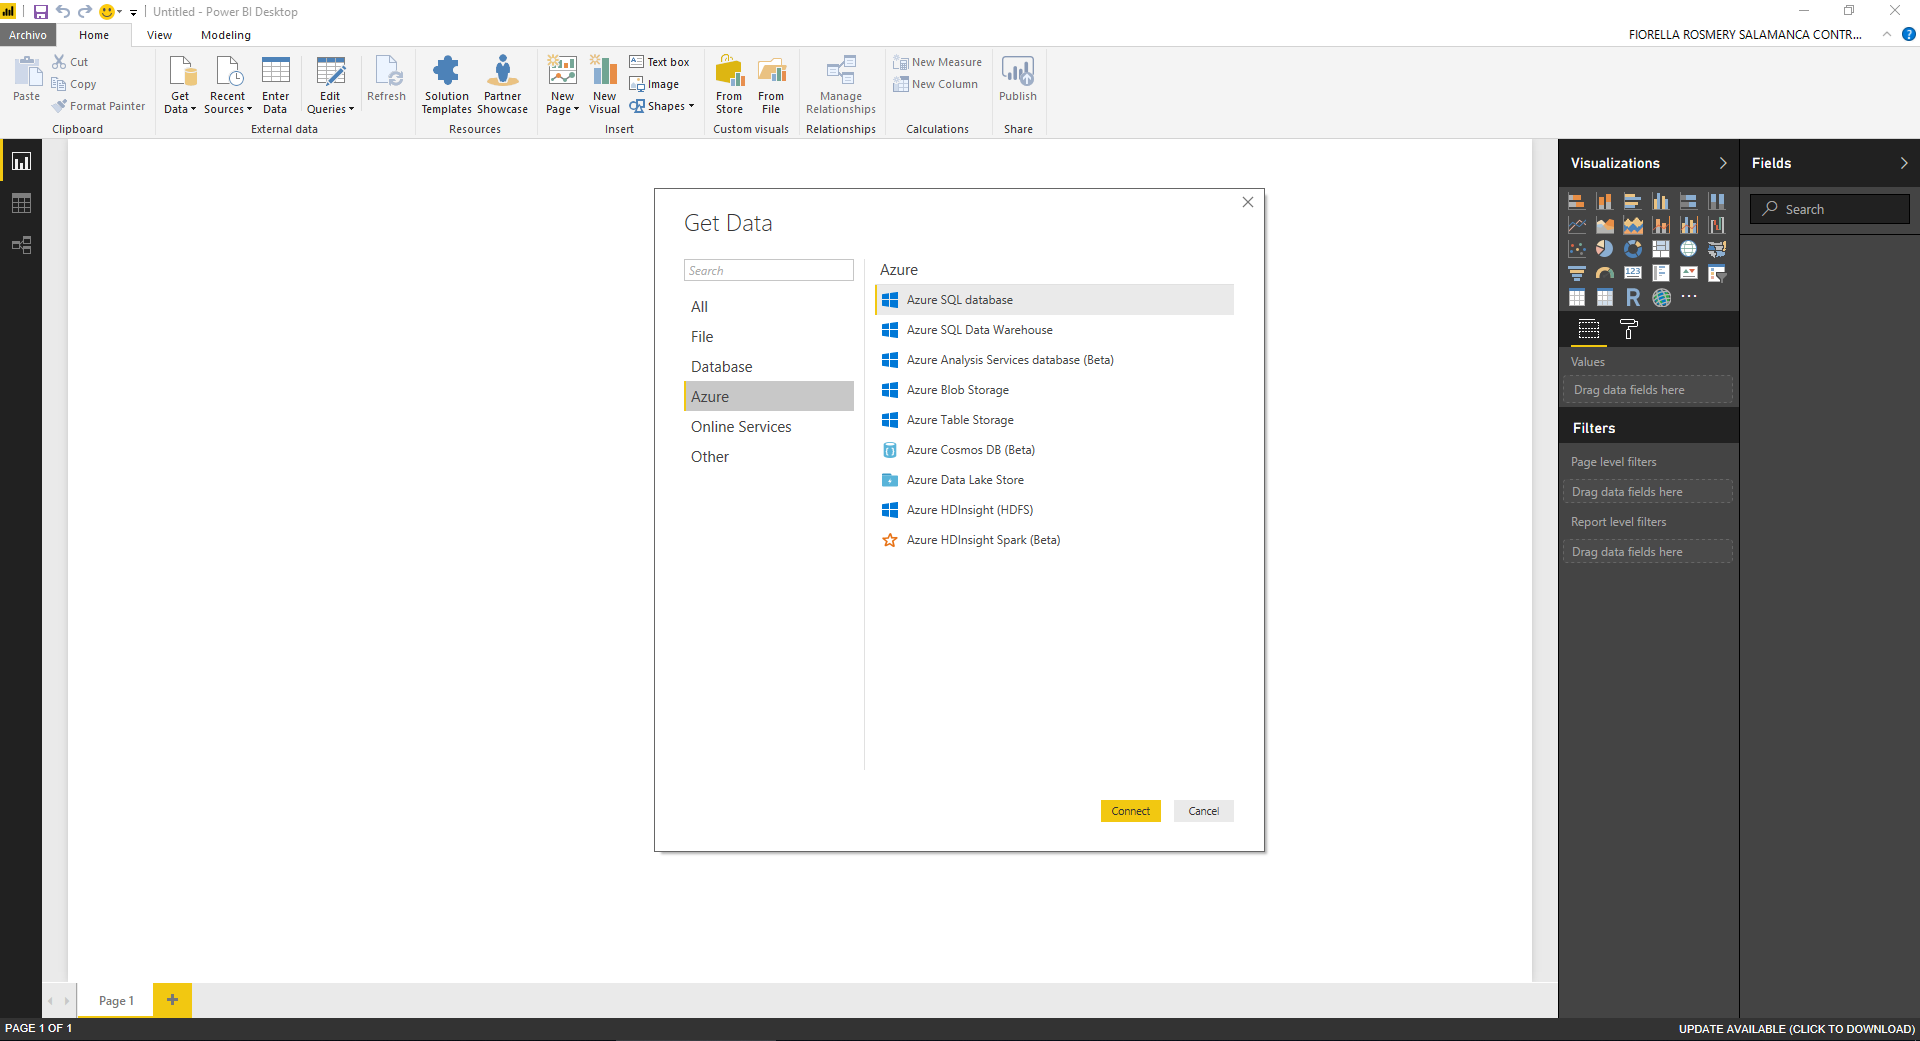
\includegraphics[width=17cm]{./Imagenes/Ejercicio1/Tarea2/4}
	\end{center}	

7. In the SQL Server database window, in the Server box, type the URL of the Azure server <Server Name>.database.windows.net.\\
8. In the Database (optional) box, type AdventureWorksLT.\\
9. Expand the Advanced options box.\\
10. In SQL Server Management Studio, copy the query under Task 1 in the Lab Exercise 1.sql query.\\
11. In Power BI Desktop, paste the query into the SQL statement (optional, requires database) box, and then click OK.\\

	\begin{center}
	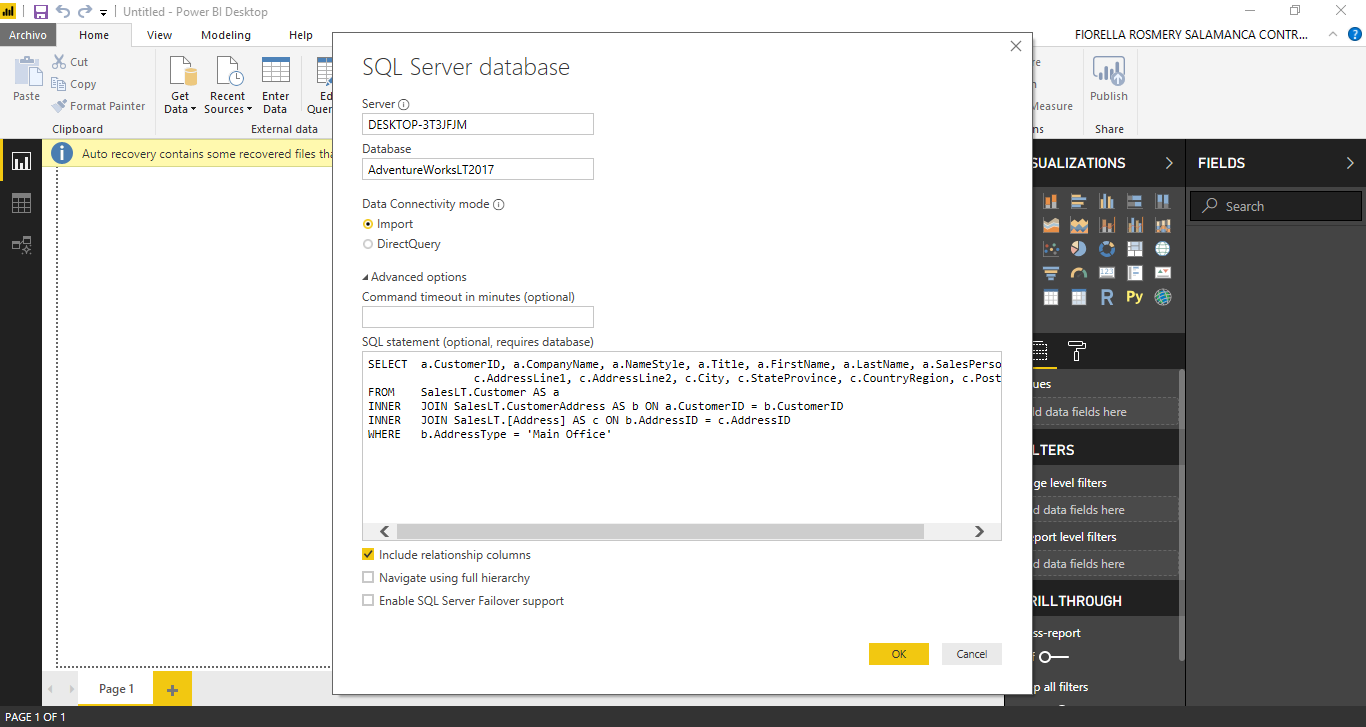
\includegraphics[width=17cm]{./Imagenes/Ejercicio1/Tarea2/5}
	\end{center}	

12. If the Access a SQL Server Database window appears, click Database, and then in the Username box, type Student, and in the Password box, type Pa\$\$w0rd. Click Connect.\\

	\begin{center}
	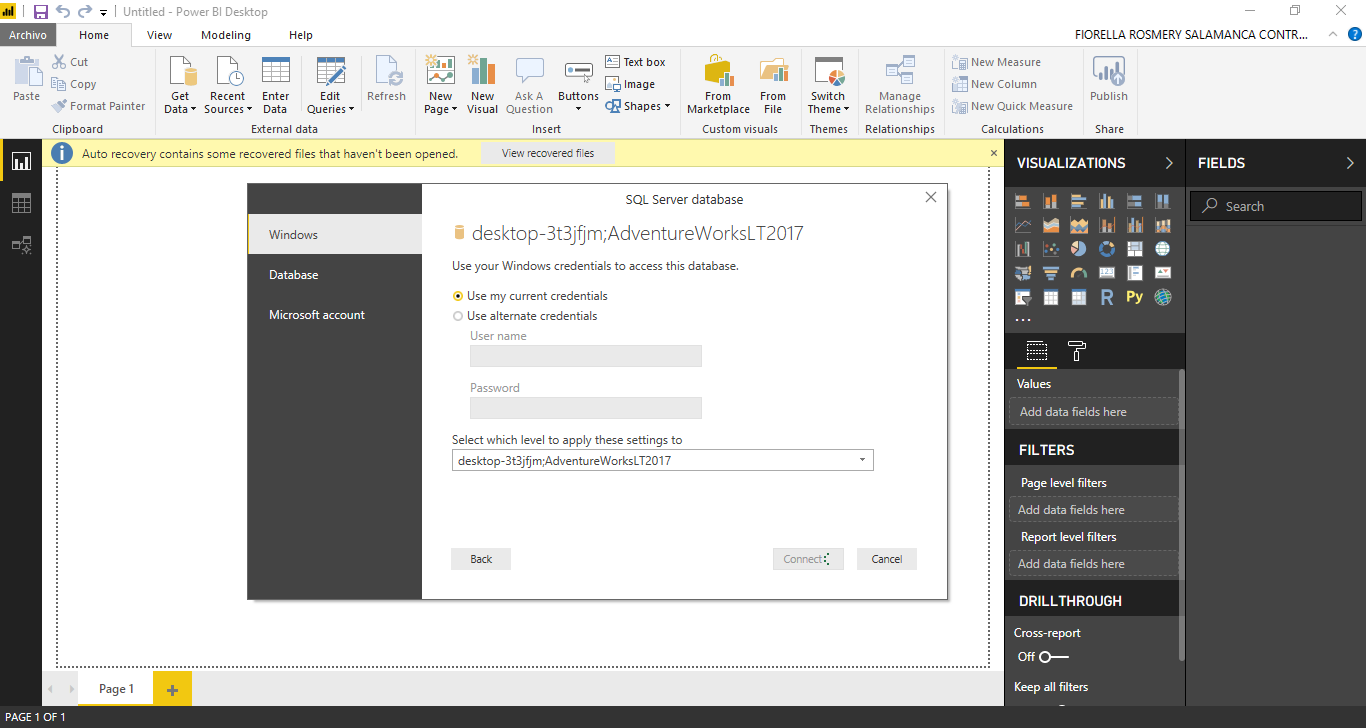
\includegraphics[width=17cm]{./Imagenes/Ejercicio1/Tarea2/6}
	\end{center}	

13. In the data preview window, click Load.\\

	\begin{center}
	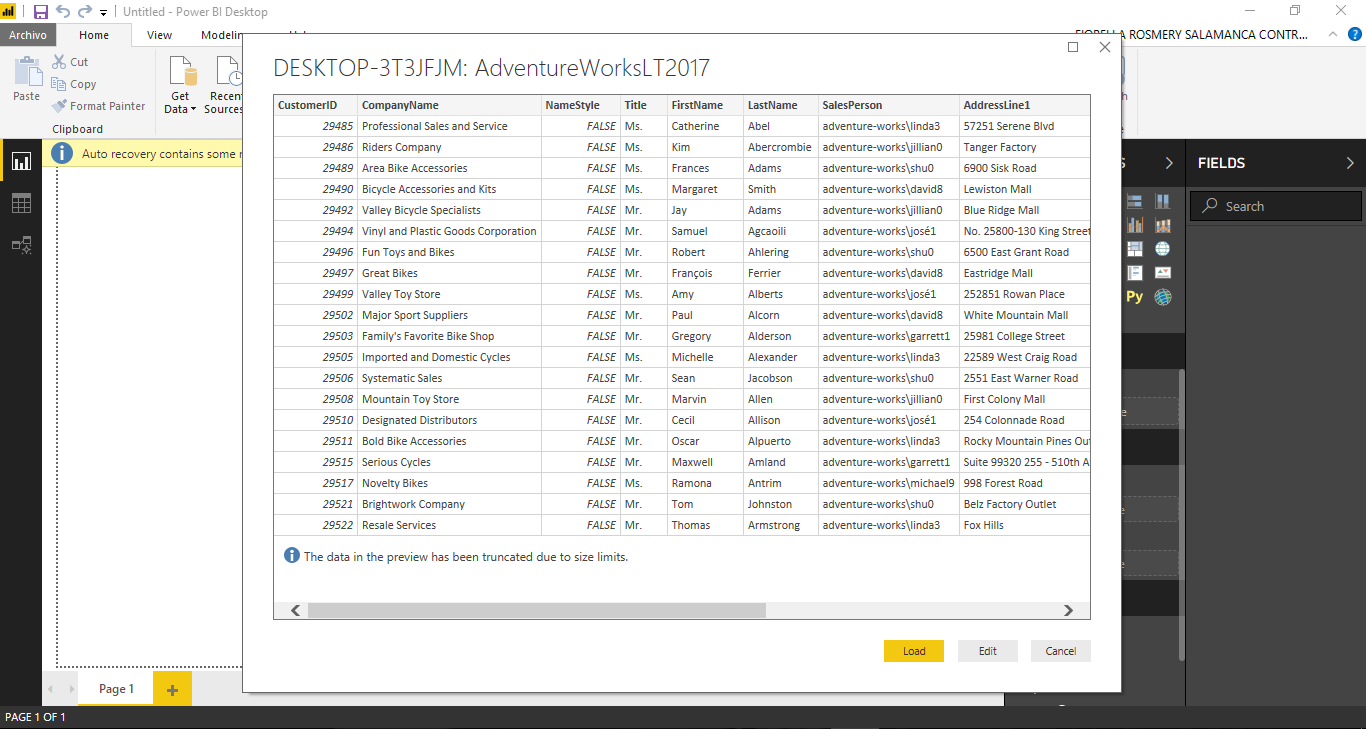
\includegraphics[width=17cm]{./Imagenes/Ejercicio1/Tarea2/7}
	\end{center}	

14. In Power BI Desktop, click Get Data then click More.\\
15. In the Get Data dialog box, click Microsoft Azure SQL database, and then click Connect.\\
16. In the SQL Server database window, in the Server box, type the URL of the Azure server <Server Name>.database.windows.net.\\
17. In the Database (optional) box, type AdventureWorksLT.\\
18. Expand the Advanced options box.\\
19. In SQL Server Management Studio, copy the query under Task 2 in the Lab Exercise 1.sql query.\\
20. In Power BI Desktop, paste the query into the SQL statement (optional, requires database) box, and then click OK.\\

	\begin{center}
	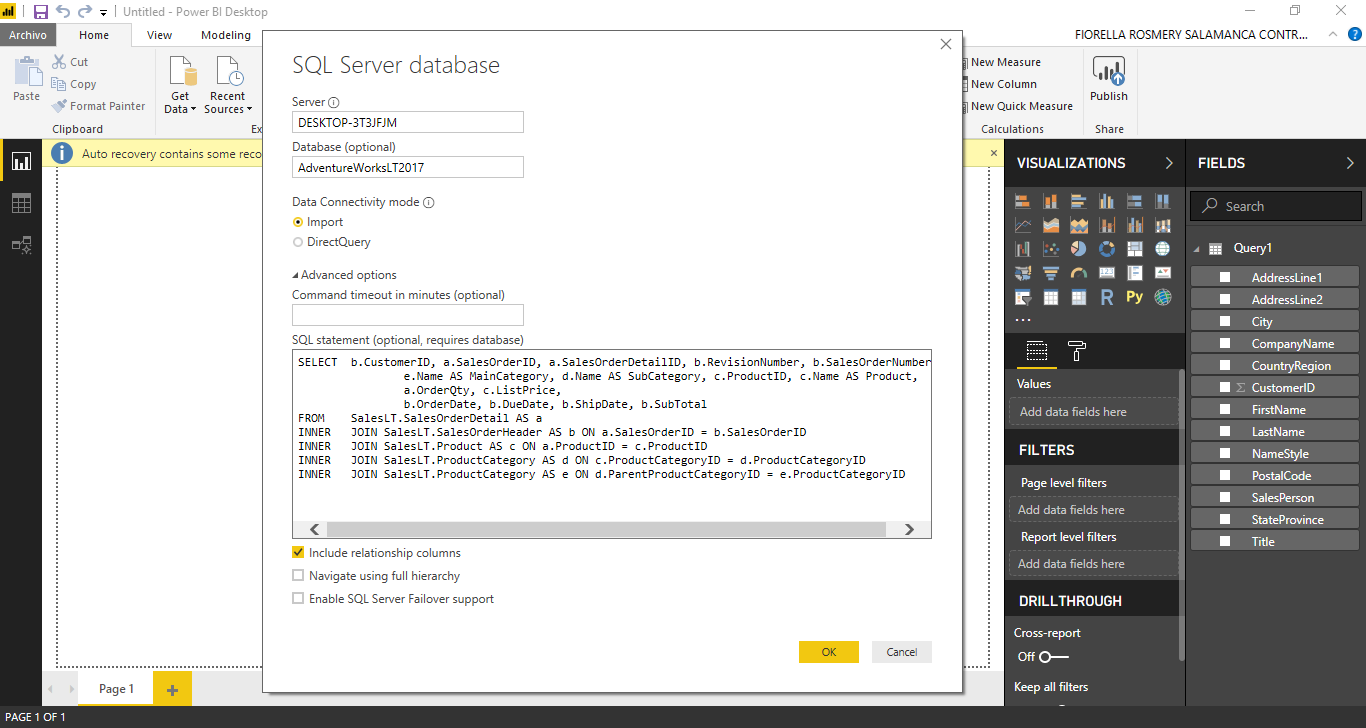
\includegraphics[width=17cm]{./Imagenes/Ejercicio1/Tarea2/8}
	\end{center}	

21. In the data preview window, click Load.\\

	\begin{center}
	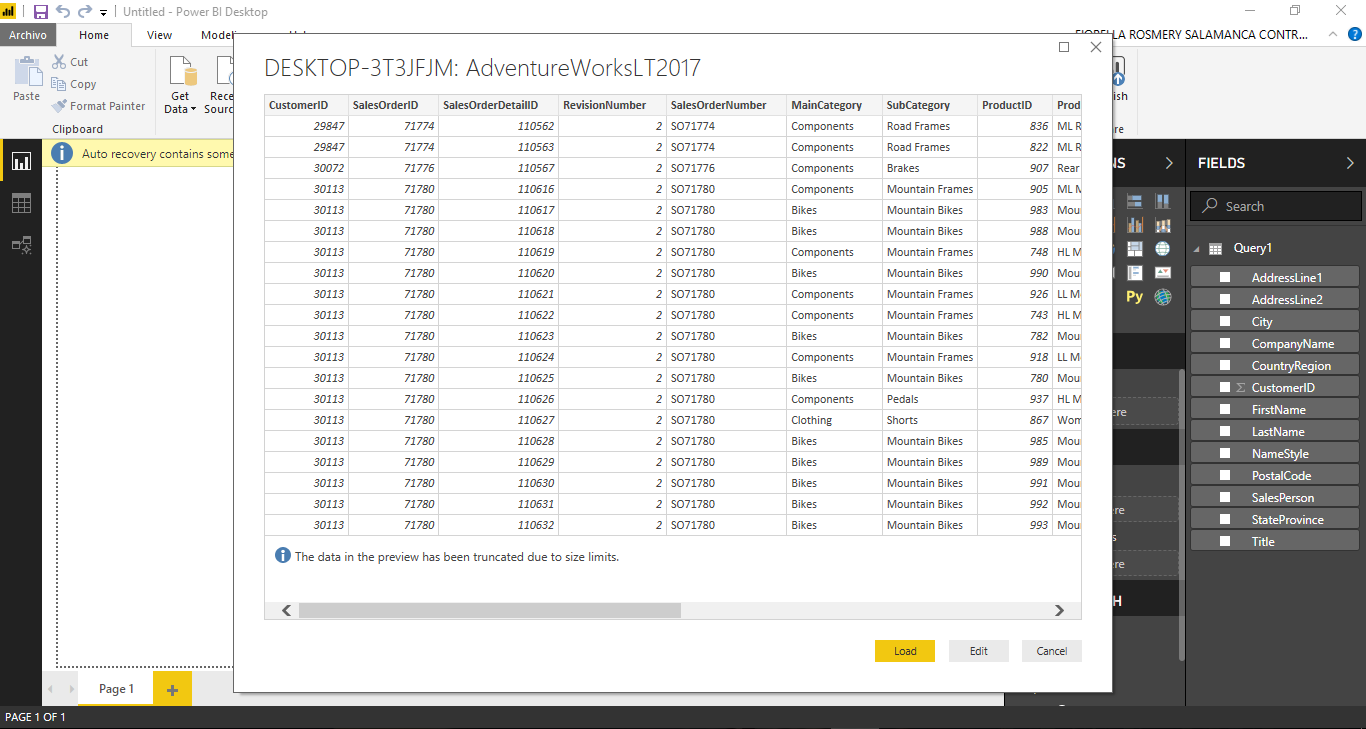
\includegraphics[width=17cm]{./Imagenes/Ejercicio1/Tarea2/9}
	\end{center}	

22. The window will close and return to the report, click Save.\\
23. In the Save As dialog box, navigate to D:/Labfiles/Lab06/Starter, in the File name box, type AdventureWorksLT Sales.pbix, and then click Save.\\

	\begin{center}
	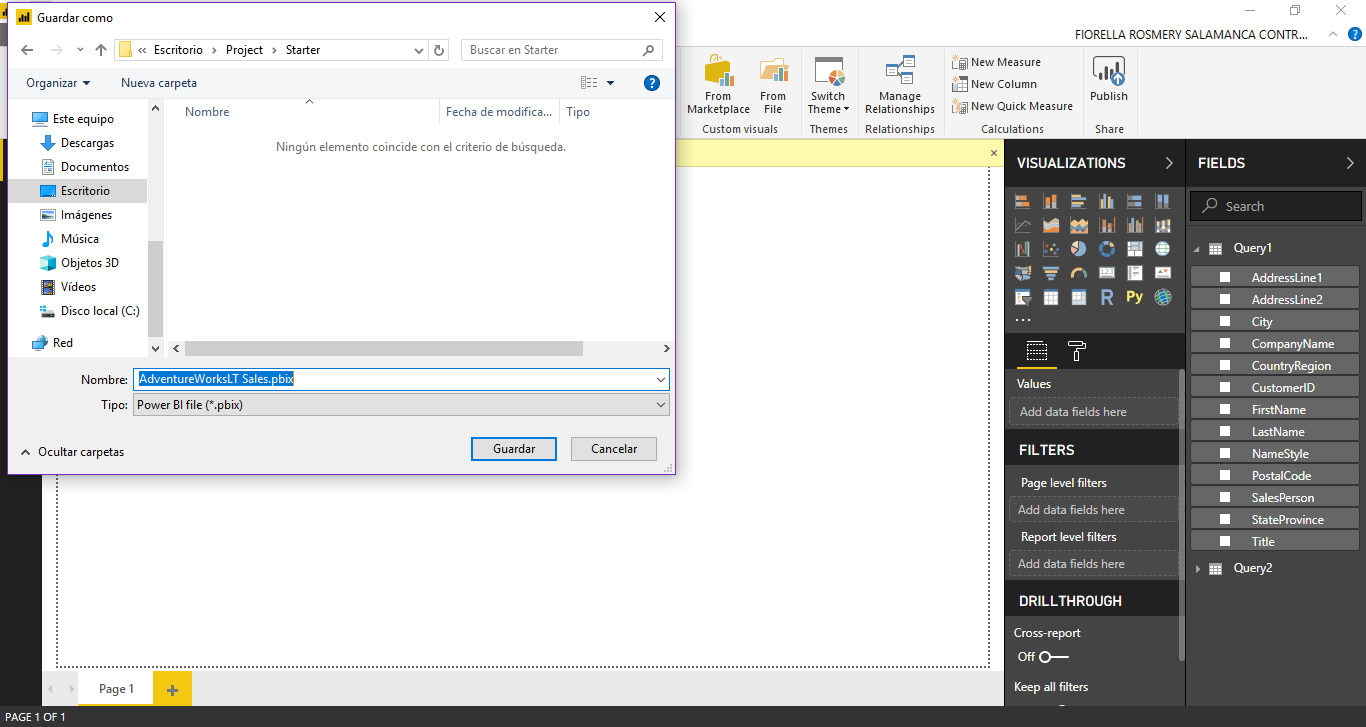
\includegraphics[width=17cm]{./Imagenes/Ejercicio1/Tarea2/10}
	\end{center}	

24. Leave Power BI Desktop open for the next task.\\